\section{Scene Modification}

	When modifying the structure of a scene graph, the objects within the scene are modified implicitly. If a scene node is re-parented to another node, the properties of the child node change. If we consider the example in Figure \ref{fig:SceneNodeReparenting1}, the \inlinecode{getLocation()} method of the \classname{Child} node will return a different value after the re-parenting.

	\begin{figure}[htbp]
		\centering
		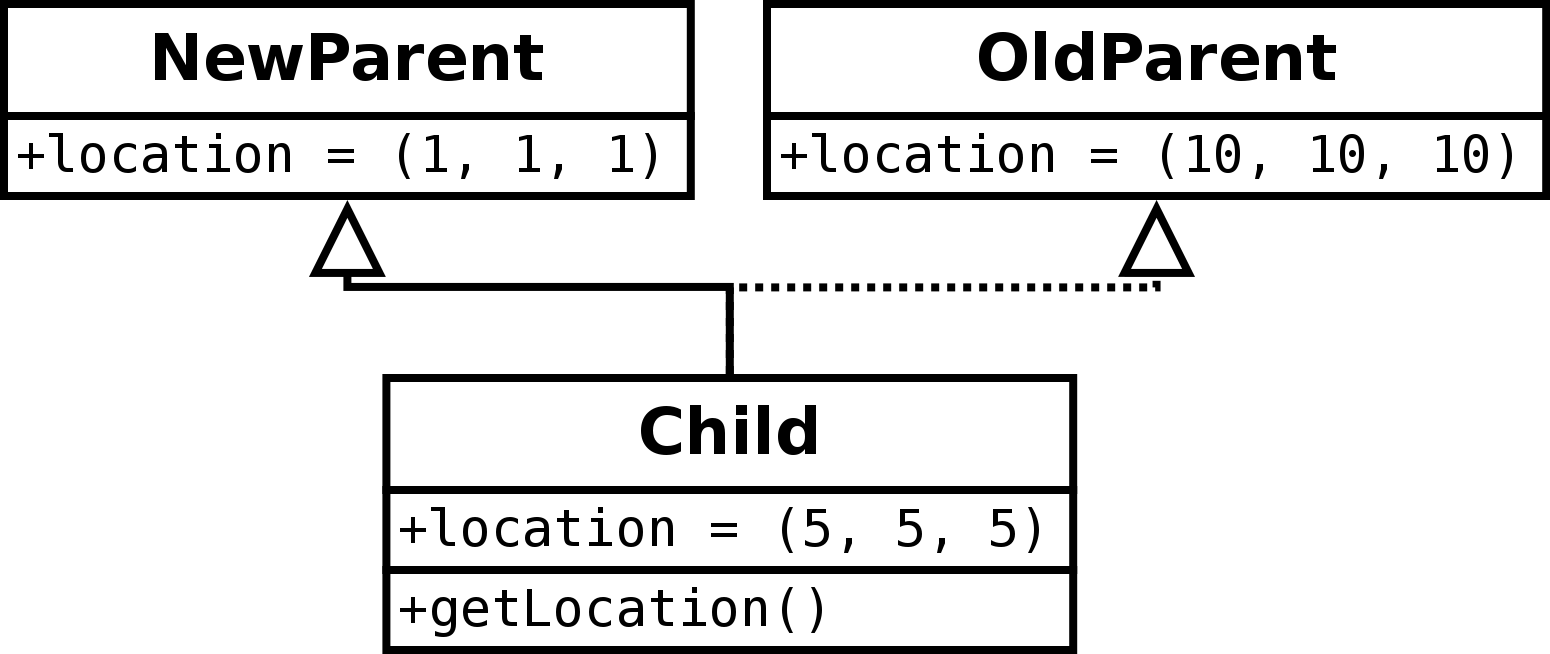
\includegraphics[width=6cm]{images/SceneNodeReparenting1.png}
		\caption{Example scene node re-parenting.}
		\label{fig:SceneNodeReparenting1}
	\end{figure}

	An object that has a \inlinecode{location} value of \vect{5}{5}{5} is positioned with that value as offset from the origin of its parent, no matter where the parent is positioned within the scene. The same is true for other properties of a scene node: rotating the \classname{TableNode} rotates all objects, updating the scale value propagates as well.

	The API needs to provide the means of keeping its property on a global scale. The object should be able to keep its location from the viewpoint of an observing camera, otherwise it will jump to another position in-between two frames. As none of our reference engines supports this operation, we will have to find a new solution.
	
	The adjustment of the object's properties is trivial from a mathematical stand point, so we could just allow the developer to pass the properties he/she wants to keep on a global scale as a parameter:

	\begin{code}[2]
		child->attachTo(newParent, POSITION | ORIENTATION);
	\end{code}

	But we had a similar problem during the design of relative rotations in Section \ref{chapter:design:coordinatesystem}. The choice at that point was to support passing arbitrary nodes as a point of reference, not limiting the developer to a set of predefined values. We will try to provide the same flexibility for this operation.

	Updating the property of a scene node while retaining its value relative to another node can be performed with these two steps:

	\begin{smalllist}
		\item The property value is queried from the viewpoint of the \emph{context node} before the object is detached from its \classname{OldParent}.
		\item The value is recalculated to match the previously queried value in the same context after the parent was changed.
	\end{smalllist}

	Finding a solution to these two operations is the foundation of the solution to the initial problem. We had already addressed the second operation in our previous discussion on relative orientation. The other operation could be performed on the same basis, leaving us with the following code sample:
	
	\begin{code}[2]
		location = child->getLocation(context);
		child->attachTo(newParent);
		child->setLocation(location, context);
	\end{code}

	We can further create a facade that updates all properties of the child node to match its previous values from the viewpoint of a context node:

	\begin{code}[2]
		child->attachTo(newParent, context);
	\end{code}

	Apart from the issues during re-arrangement of the scene graph, we will tackle another aspect of the API. We had discussed the possibility to register \classname{Task}s to be performed during the render cycle. We found that one usage scenario when getting familiar with a graphics API was the movement of objects. We were creating a separate class for updating the location of an object along a vector in each application for testing a graphics library.

	We decided to implement a dedicated \classname{Task} for this use case, as this is the most elementary form of scene modification over time. But instead of limiting the class to this single operation (movement in a single direction), we will be implementing all basic operations -- movement, rotation and scaling.

	These thoughts have led us to the design of the \classname{SceneNodeModificationTask}, which has the exact same interface as a \classname{SceneNode}. A basic class outline is shown by Figure \ref{fig:SceneNodeModificationTask}. An object of this type performs the operation repeatedly on an object as long as it is present in the main task group.

	\begin{figure}[htbp]
		\centering
		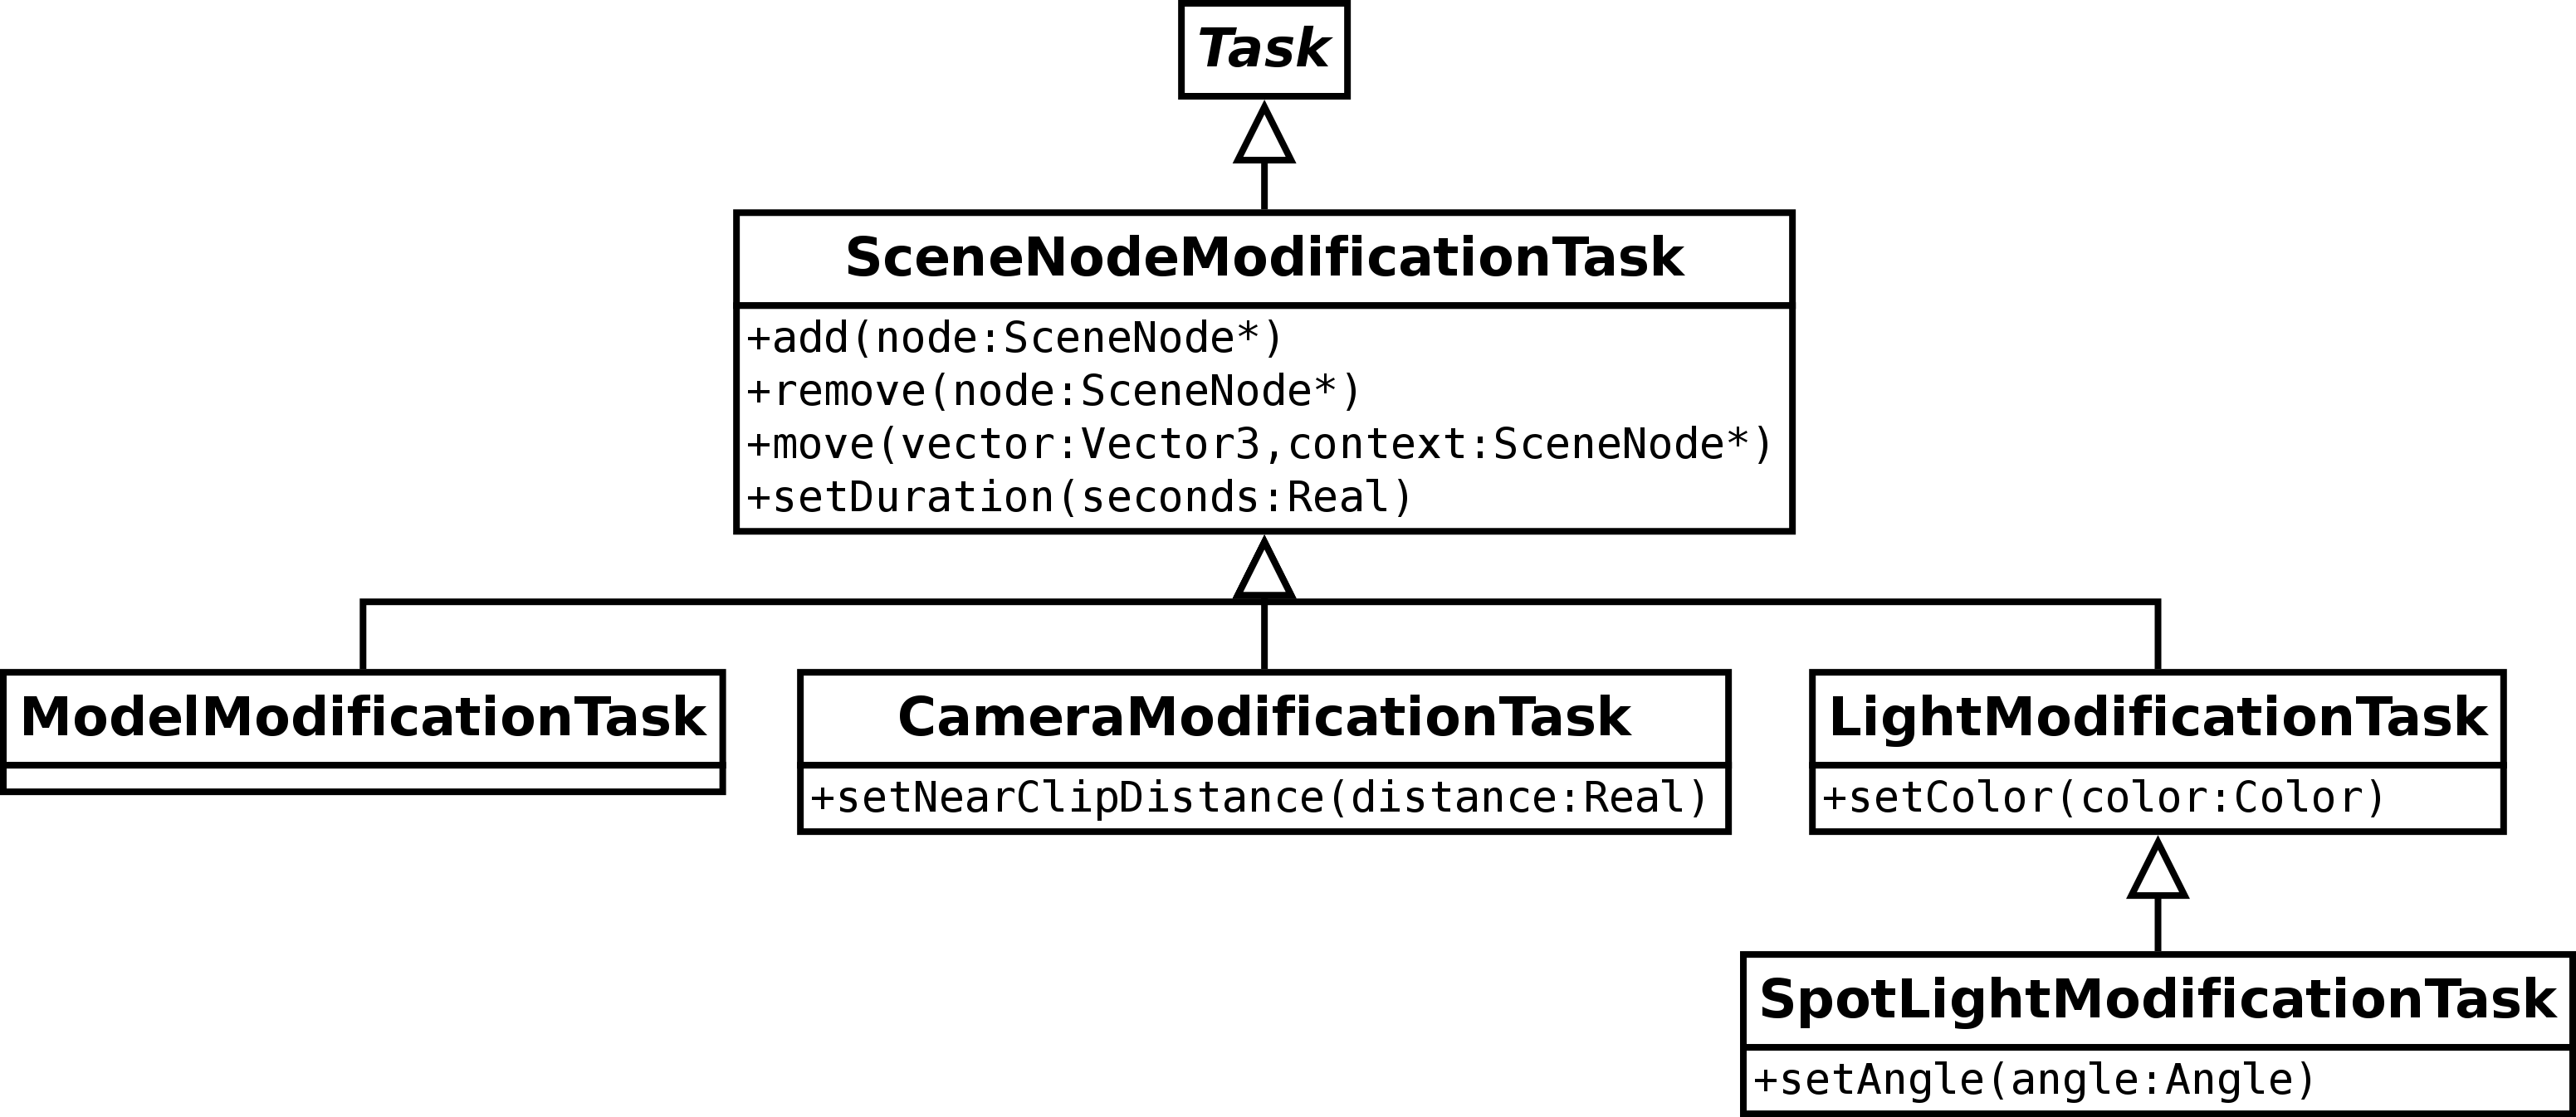
\includegraphics[width=14cm]{images/SceneNodeModificationTask.png}
		\caption{Outline of the \classname{SceneNodeModificationTask} classes. Note that the classes lack several methods that would unnecessarily clutter the diagram.}
		\label{fig:SceneNodeModificationTask}
	\end{figure}

	To configure the movement of an object along a vector, one needs to provide the vector at the length of the desired distance the object shall travel \emph{per second}. Implementing an object moving at a speed of 100 along the vector \vect{1}{1}{1} can be accomplished by the following code snippet:

	\begin{code}[2]
		task = ModelModificationTask::create();
		task->moveForward(Vector3(1, 1, 1).resize(100));
		task->register(model);
		MainTaskGroup::get()->add(task);
	\end{code}

	This \classname{Task} object will now repeatedly call the \inlinecode{moveForward()} method on the \inlinecode{model} at each loop cycle. The parameter vector will be re-sized during each call to have the correct length in relation to the time passed since its last call. The same procedure can be performed with rotations as well as scalars.

	The same concept can be applied to other properties of other objects. Dimming a spot light over the course of two seconds can be achieved with the following code:

	\begin{code}[2]
		task = LightModificationTask::create();
		task->setColor(Color::BLACK);
		task->setDuration(2);
		task->register(spotLight);
		MainTaskGroup::get()->add(task);
	\end{code}

	The implementation of these concepts are further described in Section \ref{chapter:implementation:scenegraph}.

